\chapter{A bird's eye view of OpenGL}

\section{What is OpenGL?}

At a very high level, OpenGL is a library which allows rendering of geometric shapes. This process is nowadays as good as ubiquitously accelerated by specialised hardware, commonly referred to as a GPU (Graphics Processing Unit).

You should think of OpenGL as a pipeline. You insert data on one end, and a little while later an image pops out at the other end. 

This pipeline is not a ``One Size Fits All'', however. There are a large number of settings which you are able to change which affect the final image produced. Moreover, specific components of the pipeline called ``Shaders'' are missing by default, and must be defined in order to complete the pipeline.

The number of possible ways in which the pipeline can be configured is immense. The sheer number of features can be very overwhelming when initially jumping into OpenGL. For this reason, this guide will only focus on the basics of rendering geometry and using shaders.

On the next page you can see a (somewhat simplified) overview over what the OpenGL pipeline conceptually looks like. The two mandatory Shaders have been marked with dashed lines, while ``fixed functionality'' automatically performed on the graphics card is indicated with grey boxes.

\centerline{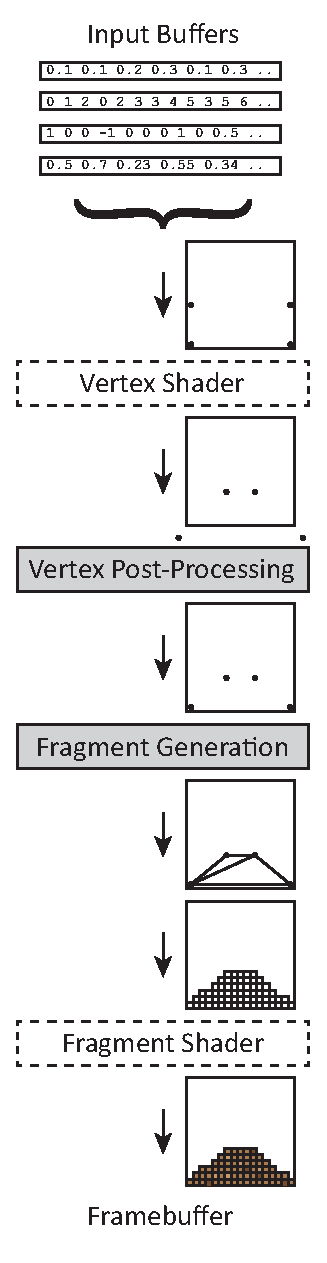
\includegraphics[scale=1.1]{images/pipeline-overview.eps}}

Let's go over each of the indicated stages in the order in which they are listed. Please keep in mind this description disregards a lot of details. 

Rendering an object starts with defining said object. OpenGL needs to know a geometric definition of the object before anything can be drawn. Objects are defined as a list of vertices (points), which can be connected into shapes such as lines or triangles. This input data resides in input buffers, which are created and filled before they can be drawn.

Once you have created and filled your input buffers, you can invoke the geometry processing pipeline by issuing so-called ``draw calls''. A draw call is a kind of transaction in which you indicate which content from your input buffers you would like to draw using the current pipeline configuration. The graphics driver will subsequently invoke the processing pipeline on the GPU and process the specified input.

The first stage of the pipeline is the execution of the vertex shader. The vertex shader is a small program which is executed in its entirety once for every single vertex rendered. Each time it is executed, it takes a vertex as input and outputs a modified vertex. The idea here is that a model can be moved around a scene or animated by applying a series of transformations on each vertex. For 3D scenes, all vertices in a scene must be transformed every frame.

Once all vertices have been processed by an instance of the vertex shader, some additional processing is necessary. Amongst others, clipping is performed as well as the viewport transform. We'll return to clipping specifically a little later, because it's a key part of understanding what you're doing when drawing objects in OpenGL.

Now that the vertex positions are known, vertices can be connected together to form shapes, most commonly triangles. These shapes are in turn rasterised into pixels. The diagram specifically shows what this looks like for triangles. The vertex post-processing and rasterisation is usually all done in hardware on the graphics processor. You don't have to do any of that yourself.

The second mandatory shader in the pipeline is the ``fragment shader''. It takes a rasterised pixel as input, and is responsible for assigning a colour to it. It is executed once for each rasterised pixel. The word ``fragment'' in OpenGL is used to describe a rasterised pixel which is being drawn, but may not necessarily end up being shown in the final image. This can for example happen if another piece of geometry is drawn over the fragment at a later time while rendering the frame. 

The final output is written to a so-called framebuffer. The framebuffer is either directly or indirectly (in case of a windowing system) sent to a monitor to be displayed.

\section{The ClipBox}

As mentioned previously, I'd like to put special emphasis on the clipping process, because it is vital for understanding what is going on when rendering geometry.

Clipping is essentially the process of throwing away all geometry which exceeds the bounds of the screen. If a shape only partially sticks out of the clipping volume, it is cut down exactly to fit within the clipping volume. Clipping also ensures that objects behind the camera are not visible in the rendered image. 

In OpenGL, the clipping volume is defined to be a cube around the origin, which ranges between the values of -1 and 1 along each major axis.

The vertex shader is responsible for compressing the entire contents of your scene into this little 2x2x2 cube, no matter how large the dimensions of your scene are. Anything outside of it will not appear on screen.

Moreover, there is one particular side of this clipbox which has been defined to be the side from which you as a viewer look into the box at the scene you're rendering. The OpenGL standard defines this side to the one on the side of the \emph{negative z-axis} looking into the \emph{positive} direction. 

Here is a visualisation of the clipbox, with the aforementioned viewing side highlighted:

\vspace{0.5cm}
\centerline{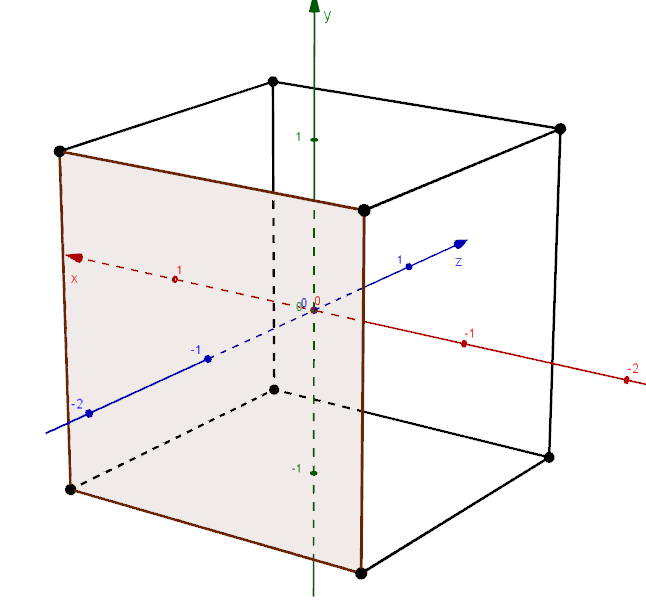
\includegraphics[scale=0.7]{images/clipbox_corrected.png}}
\newpage
\section{OpenGL functions}

The design of OpenGL at its core is that of a state machine. When starting your application, you create a so-called ``OpenGL context''. After doing so, you issue commands to the context by calling OpenGL functions. These functions cause state within the context to change, hence the state machine designation. 

You should think of this state as all data and settings necessary for configuring the OpenGL pipeline. You set up the pipeline in such a way that it will draw the object you want in the way you would like it to. When ready, you issue a draw call and the object is rendered by the pipeline.

Using this style of API may be somewhat counter-intuitive if you've never interacted with such an interface before. However, in practice main difference with more ``conventional'' libraries is that you don't create any data structures or objects yourself. Instead, you give commands to OpenGL which causes the objects to be created for you inside the context. You can subsequently use other functions to modify these objects.

As you will see in later chapters of this guide, setting up various kinds of OpenGL state often implies calling a series of functions in a specific order, rather than issuing a single command. 

OpenGL functions have a very distinct format, making them very easy to distinguish. Here's an example:

\begin{minted}{c}
void glUniform4f(int location, float v0, float v1, float v2, float v3);
\end{minted}

What this function does is not very relevant at this point. Instead, notice the ``gl'' prefix, which is common to all OpenGL functions. 

In some cases a function also allows you to specify the datatype and the number of operands if multiple values are allowed. These functions contain type modifiers at the end of their name, such as the one shown above. In this case, the ``4'' indicates you'd like to pass 4 values, and the ``f'' indicates you're passing in values with a floating point datatype. 

Similarly, the function \mintinline{c}{glUniform3i()} indicates you'll pass in 3 integer values.

Looking up an OpenGL function in the documentation will show you all possible combinations of type modifiers of that particular function.

I want to make one note on the functions listed in this guide. The OpenGL documentation commonly lists rather cryptic data types for each of the parameters. For the sake of being able to understand them, I changed them to those you will be most commonly calling these functions with. If you want the official specifications, I recommend using the official online documentation pages.